\documentclass{article}
\usepackage{graphicx}
\usepackage{pgfplots}
\usepackage{tikz}
\usepackage{amsmath}
\usepackage{amssymb}

\pgfplotsset{compat=1.18}
\usepgfplotslibrary{fillbetween}

\title{Reflection Principle}
\author{Jongkook Choi}
\date{\today}
\begin{document}

\maketitle

\section{Brownian bridge}

Setup
\begin{itemize}
    \item log-price $X_t$ follows BM $dX = \mu' dt + \sigma dW$
          \begin{itemize}
              \item Where  $\mu' = \mu - \frac{1}{2} \sigma^2$ and $dS = S(\mu dt + \sigma dW)$
          \end{itemize}
    \item $M = \sup_{0 \le t \le T} X_t$.
\end{itemize}
~\\
Useful equations
\begin{itemize}
    \item $P\left(M(t_1)=m|X(t_0)=x_0\right) \sim \textrm{Rayleigh}\left(\sigma \sqrt{t_1-t_0}\right) $
    \item $P\left(M(t_1)=m|X(t_0)=x_0, X(t_1)=x_1\right) =  \exp \left( - \frac{2(m - x_0)(m - x_1)}{\sigma^2 (t_1-t_0)} \right)$
          \begin{itemize}
              \item Reflection principle can be used to prove this.
          \end{itemize}
\end{itemize}
~\\
Thinking about $\sigma = 1, \mu' = 0$ is enough.
It is because Girsanov theorem ensures that the process is still a Brownian motion under dirftless measure.

It is convenient that the Girsanov factor cancels out.
% $$
\begin{gather*}
    P^\mathbb{P}\left(M(t_1)=m|X(t_0)=x_0, X(t_1)=x_1\right) \\
    =
    \frac
    {P^\mathbb{P}\left(M(t_1)=m, X(t_1)=x_1| X(t_0)=x_0\right)}
    {P^\mathbb{P}\left(X(t_1)=x_1\right)| X(t_0)=x_0} \\
    =
    \frac
    {P^\mathbb{P}\left(M(t_1)=m, X(t_1)=x_1|\mathcal{F}_{t_0}\right)}
    {P^\mathbb{P}\left(X(t_1)=x_1|\mathcal{F}_{t_0}\right)}\\
    =
    \frac
    {P^\mathbb{Q}\left(M(t_1)=m, X(t_1)=x_1|\mathcal{F}_{t_0}\right) \frac{d\mathbb{P}}{d\mathbb{Q}}}
    {P^\mathbb{Q}\left(X(t_1)=x_1|\mathcal{F}_{t_0}\right) \frac{d\mathbb{P}}{d\mathbb{Q}}}\\
    =
    \frac
    {P^\mathbb{Q}\left(M(t_1)=m, X(t_1)=x_1|\mathcal{F}_{t_0}\right)}
    {P^\mathbb{Q}\left(X(t_1)=x_1|\mathcal{F}_{t_0}\right)}\\
    =
    P^\mathbb{Q}\left(M(t_1)=m|X(t_0)=x_0, X(t_1)=x_1\right)
\end{gather*}
\section{Reflection Principle}

Let us consider $dX = dW$.

The following figure shows two distribution
\begin{itemize}
    \item Solid line (left) : $X(t)$, $X(t_0) = x_0$, $X(t_1) = x_1$
    \item Dashed line (right) : $X^*(t)$, $X^*(t_0) = 2m - x_0$, $X^*(t_1) = 2m-x_1$
\end{itemize}

\begin{figure}[htbp]
    \centering
    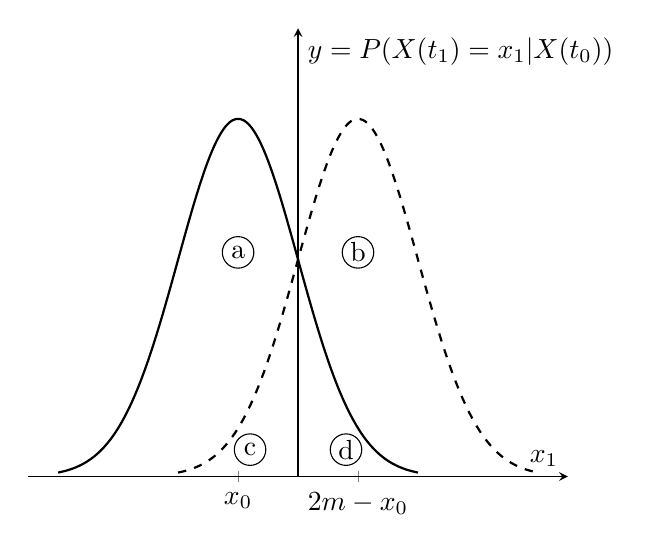
\begin{tikzpicture}
        \begin{axis}[
                axis lines=middle,
                xmin=-4.5, xmax=4.5,
                ymin=0, ymax=0.5,
                xtick={-1, 0., 1},
                xticklabels={$x_0$, $m$, $2m-x_0$},
                ytick=\empty,
                xlabel={$x_1$},
                ylabel={$y = P(X(t_1)=x_1|X(t_0))$},
                clip=false
            ]

            % Define the two normal distributions (Mean = -1 and Mean = 2)
            \addplot[name path=A, domain=-4:2, samples=100, thick, smooth]
            {exp(-(x+1)^2/2) / sqrt(2*pi)};
            \addplot[name path=B, domain=-2:4, samples=100, dashed, thick, smooth]
            {exp(-(x-1)^2/2) / sqrt(2*pi)};

            % Labels for specific points/regions inside the plot
            \draw (axis cs: -1, 0.25) circle [radius=0.2cm] node {a};
            \draw (axis cs: 1, 0.25) circle [radius=0.2cm] node {b};
            \draw (axis cs: -0.8, 0.03) circle [radius=0.2cm] node {c};
            \draw (axis cs: 0.8, 0.03) circle [radius=0.2cm] node {d};

        \end{axis}
    \end{tikzpicture}
    \caption{$X^*(t)$(dashed line) is a mirror image of $X(t)$(solid line). \\
        (a) and (d) represents area under $X(t)$(solid line)\\
        (c) and (b) represents area under $X^*(t)$(dashed line)
    }
    % \label{fig:reflection_principle}
\end{figure}

\begin{itemize}
    \item When there is no bouncy wall placed at $m$
          \begin{itemize}
              \item (a) : $P(X(t_1) \le m | X(t_0) = x_0, X(t_1) = x_1)$,
              \item (d) : $P(X(t_1) \ge m | X(t_0) = x_0, X(t_1) = x_1)$
          \end{itemize}
    \item When there is a bouncy wall placed at $m$
          \begin{itemize}
              \item (a) : $P( 1 | X(t_0) = x_0, X(t_1) = x_1)$
              \item \textbf{\color{red} (a)-(c) = (a)-(d) }: $\color{red}P(M(t_1) < m | X(t_0) = x_0, X(t_1) = x_1)$
              \item (c) : $P(M(t_1) = m | X(t_0) = x_0, X(t_1) = x_1)$ (touched wall)
          \end{itemize}
\end{itemize}

It makes sense because, starting from $x_0$ and hitting the wall is equivalent to starting from $2m - x_0$ and crossing the wall.

\textbf{\color{red} Be careful, the point can cross(bounce) the wall multiple times.}
However, it does not matter because due to the symmetry, we can flip the cases that crosses the line odd times.


\end{document}

\end{document}